\section{Probability Using Tree Diagrams}

In this section you will learn to:
\begin{enumerate}
    \item Use probability trees to organize information in probability problems
    \item Use probability trees to calculate probabilities
\end{enumerate}

As we have already seen, tree diagrams play an important role in solving probability problems. A tree diagram helps us not only visualize, but also list all possible outcomes in a systematic fashion. Furthermore, when we list various outcomes of an experiment and their corresponding probabilities on a tree diagram, we gain a better understanding of when probabilities are multiplied and when they are added.

The meanings of the words "and" and "or" become clear when we learn to multiply probabilities horizontally across branches, and add probabilities vertically down the tree.

Although tree diagrams are not practical in situations where the possible outcomes become large, they are a significant tool in breaking the problem down in a schematic way. We consider some examples that may seem difficult at first, but with the help of a tree diagram, they can easily be solved.

\begin{example}
    A person has four keys and only one key fits the lock of a door. What is the probability that the locked door can be unlocked in at most three tries?
\end{example}

\begin{solution}
    Let U be the event that the door has been unlocked and L be the event that the door has not been unlocked. Since there is only one correct key out of four, the probability of not unlocking the door with one try is \( \frac{3}{4} \). The probability of not unlocking the door in three tries is \( \left(\frac{3}{4}\right)^3 \). Therefore, the probability of unlocking the door in at most three tries is the complement:
    \[ P(U) = 1 - P(L) = 1 - \left(\frac{3}{4}\right)^3 = 1 - \frac{27}{64} = \frac{37}{64} \]


    \begin{center}
        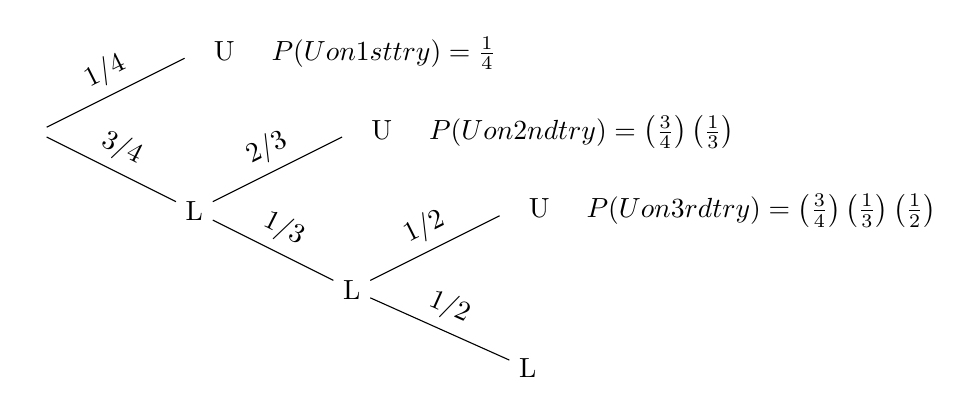
\begin{tikzpicture}[grow=right, sloped]
            \tikzstyle{level 1}=[level distance=2cm, sibling distance=2cm]
            \tikzstyle{level 2}=[level distance=2cm, sibling distance=2cm]
            \tikzstyle{level 3}=[level distance=2cm, sibling distance=2cm]
            \tikzstyle{level 4}=[level distance=2cm, sibling distance=2cm]
            % Level 1
            \node {}
            child {
            node {L}
            child {
            node {L}
            child {
                    node[right] {L}
                    edge from parent
                    node[above] {1/2}
                }
            child {
            node [label=right: {U \quad $P(U \text{on 3rd try}) = \left(\frac{3}{4}\right)\left(\frac{1}{3}\right)\left(\frac{1}{2}\right)$}]{}
            % node[right] {U \quad $P(U \text{on 3rd try}) = \left(\frac{3}{4}\right)\left(\frac{1}{3}\right)\left(\frac{1}{2}\right)$}
            edge from parent
            node[above] {1/2}
            }
            edge from parent
            node[above] {1/3}
            }
            child {
            % node[right] {U \quad $P(U \text{on 2nd try}) = \left(\frac{3}{4}\right)\left(\frac{1}{3}\right)$}
            node [label=right: {U \quad $P(U \text{on 2nd try}) = \left(\frac{3}{4}\right)\left(\frac{1}{3}\right)$}]{}
            edge from parent
            node[above] {2/3}
            }
            edge from parent
            node[above] {3/4}
            % node[below] {P(U on 1st try) = 1/4}
            }
            child {
            node [label=right: {U \quad $P(U \text{on 1st try}) = \frac{1}{4}$}]{}
            % node {U \quad $P(U \text{on 1st try}) = \frac{1}{4}$}
            edge from parent
            node[above] {1/4}
            };
        \end{tikzpicture}
    \end{center}
    The probability of unlocking the door in the first try \( = \frac{1}{4} \)

    The probability of unlocking the door in the second try \( = \left(\frac{3}{4}\right)\left(\frac{1}{3}\right) = \frac{1}{4} \)

    The probability of unlocking the door in the third try \( = \left(\frac{3}{4}\right)\left(\frac{2}{3}\right)\left(\frac{1}{2}\right) = \frac{1}{4} \)

    Therefore, the probability of unlocking the door in at most three tries \( = \frac{1}{4} + \frac{1}{4} + \frac{1}{4} = \frac{3}{4}. \)

\end{solution}

\begin{example}
    A jar contains 3 black and 2 white marbles. We continue to draw marbles one at a time until two black marbles are drawn. If a white marble is drawn, the outcome is recorded and the marble is put back in the jar before drawing the next marble. What is the probability that we will get exactly two black marbles in at most three tries?
\end{example}

\begin{solution} Starting with a tree diagram

    \begin{tikzpicture}[grow=right, sloped]
        \tikzstyle{level 1}=[level distance=2cm, sibling distance=6cm]
        \tikzstyle{level 2}=[level distance=2cm, sibling distance=4cm]
        \tikzstyle{level 3}=[level distance=2cm, sibling distance=2cm]
        \tikzstyle{level 4}=[level distance=2cm, sibling distance=1cm]
        % Level 1
        \node {}
        child {
        node {W}
        child {
        node {B}
        child {
                node[right] {W}
                edge from parent
                node[above] {2/4}
            }
        child {
        node [label=right: {$B \quad P(WBB)=(2/5)(3/5)(2/4)=3/25$}]{}
        edge from parent
        node[above] {2/4}
        }
        edge from parent
        node[above] {3/5}
        }
        child {
        node [label=right: {W}]{}
        edge from parent
        node[above] {2/5}
        }
        edge from parent
        node[above] {2/5}
        }
        child {
        node {B}
        child {
        node {W}
        child {
                node[right] {W}
                edge from parent
                node[above] {2/4}
            }
        child {
        node [label=right: {$B \quad P(BWB)=(3/5)(2/4)(2/4)=3/20$}]{}
        edge from parent
        node[above] {2/4}
        }
        edge from parent
        node[above] {2/4}
        }
        child {
        node [label=right: {$B \quad P(BB)=(3/5)(2/4)=3/10$}]{}
        edge from parent
        node[above] {2/4}
        }
        edge from parent
        node[above] {3/5}
        };
    \end{tikzpicture}
    The probability that we will get two black marbles in the first two tries is listed adjacent to the lowest branch, and it is \( \frac{3}{10} \).

    The probability of getting first black, second white, and third black = \( \frac{3}{20} \).

    Similarly, the probability of getting first white, second black, and third black = \( \frac{3}{25} \).

    Therefore, the probability of getting exactly two black marbles in at most three tries = \( \frac{3}{10} + \frac{3}{20} + \frac{3}{25} = \frac{57}{100} \).


\end{solution}

\begin{example}
    A circuit consists of three resistors: resistor \( R_1 \), resistor \( R_2 \), and resistor \( R_3 \), joined in a series. If one of the resistors fails, the circuit stops working. The probabilities that resistors \( R_1 \), \( R_2 \), or \( R_3 \) will fail are 0.07, 0.10, and 0.08, respectively. Find the probability that at least one of the resistors will fail.
\end{example}
\begin{solution}
    The probability that at least one of the resistors fails is \( 1 - \) none of the resistors fails. We don't even need to draw a tree because we can visualize the only branch of the tree that assures this outcome.

    The probabilities that \( R_1 \), \( R_2 \), \( R_3 \) will not fail are \( 0.93 \), \( 0.90 \), and \( 0.92 \) respectively. Therefore, the probability that none of the resistors fails is
    \[ (0.93)(0.90)(0.92) = 0.77 \]
    Thus, the probability that at least one of them will fail is \[ 1 - 0.77 = 0.23 \].
\end{solution}
